\documentclass[10pt,a4paper]{article}
\usepackage[margin=18mm]{geometry}\usepackage{fontspec,amsmath,graphicx,booktabs}
\setmainfont{Latin Modern Roman}\setlength{\parindent}{0pt}\setlength{\parskip}{6pt}
\begin{document}
{\LARGE Corrected final-reference correspondence}\par 6 October 2026

\textbf{Correction to earlier reports.} The final channel-averaged trajectory was not uniformly spaced in anisotropy, although its constituent cycles had equal-guide-arc bins. Matching that final reference at uniform index fractions was incorrect. This report supersedes the previous equal-arc forward-fit comparisons, including the forward part of the complex/inverse-circle report. The inverse-circle collapse counterexample is independent of this error.

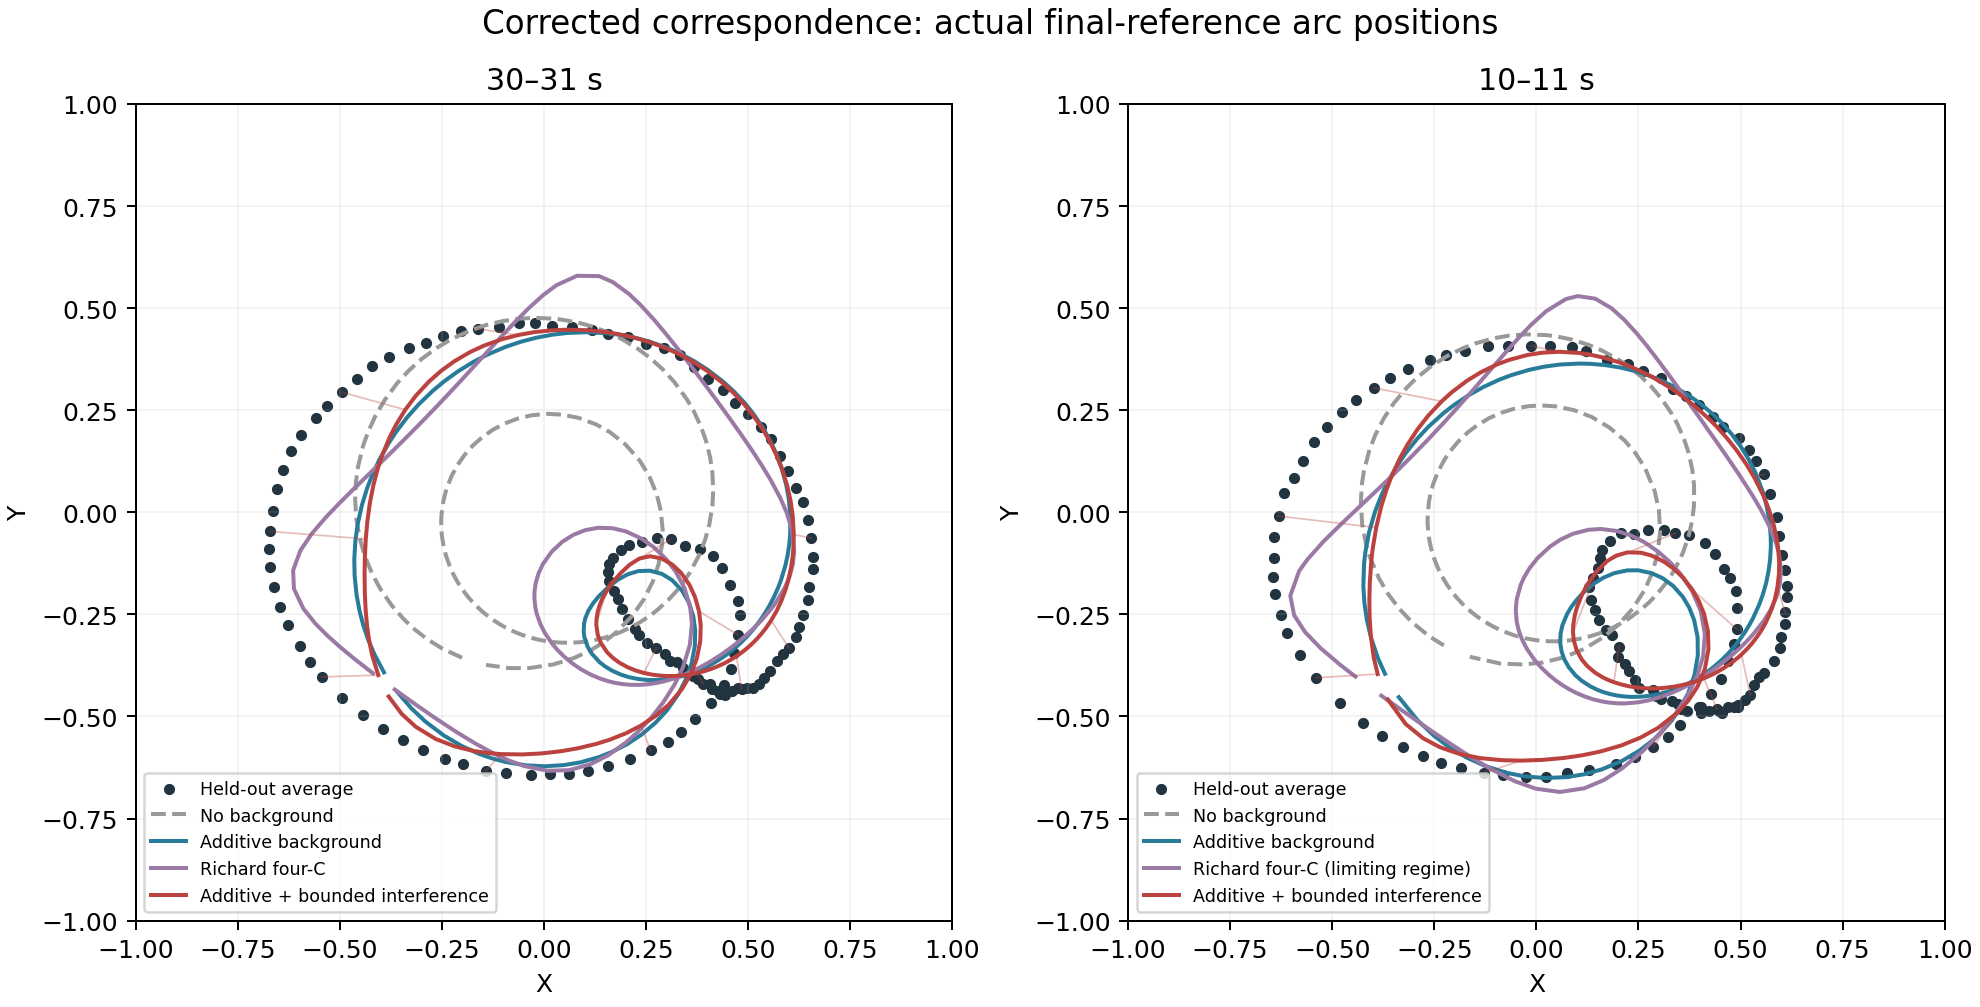
\includegraphics[width=\linewidth]{corrected_fits.png}

Observed points are intentionally unchanged and therefore remain nonuniformly spaced. The model is now evaluated at their actual training-reference arc fractions. Thin red segments join selected corresponding observed and predicted points; no nearest-neighbour matching is used.

\begin{tabular}{llrrrr}\toprule
Window & Model & Channel RMS & XY RMS & BG/\(T_{\max}\) & \(\theta\) range\\\midrule
30s & None & 0.08281 & 0.41166 & 0.0\% & 29.0--44.4$^\circ$ \\
30s & Additive & 0.02902 & 0.11611 & 37.3\% & 29.4--90.0$^\circ$ \\
30s & Richard four-C & 0.03930 & 0.15151 & --- & 28.9--89.0$^\circ$ \\
30s & Additive + interference & 0.02670 & 0.10775 & 45.7\% & 30.3--90.0$^\circ$ \\
10s & None & 0.08242 & 0.41597 & 0.0\% & 30.3--41.9$^\circ$ \\
10s & Additive & 0.03333 & 0.13886 & 40.3\% & 33.8--89.8$^\circ$ \\
10s & Richard four-C$^*$ & 0.03973 & 0.15963 & --- & 33.4--89.0$^\circ$ \\
10s & Additive + interference & 0.02987 & 0.12507 & 43.8\% & 34.7--90.0$^\circ$ \\
\bottomrule\end{tabular}

$^*$Richard's 10 s row is a limiting regime with vanishing signal brightness and growing coefficients; it is not a stable finite-coefficient correction. No physical background power is inferred from Richard's approximation. All angular ranges are conditional model outputs, not independently validated angles.
\newpage
{\Large What changed, and how it was checked}

For each final training track, interpolate the four intensities together along the closed, ordered list of bins. Calculate X/Y from this channel interpolant, integrate its arc length, and record the fraction \(u_k\) at each original bin. A candidate full measured-model curve is then evaluated at fractions \((\delta\pm u_k)\bmod1\), with one fitted cyclic offset and both directions tested.

The held-out track uses exactly the training-derived \(u_k\), offset, direction and fitted physical parameters. It is not independently reparameterized. This preserves every original observed channel value and the original equal-bin intensity weighting. It is not a new uniformly reweighted reference; uniform resampling would additionally change the objective weights.

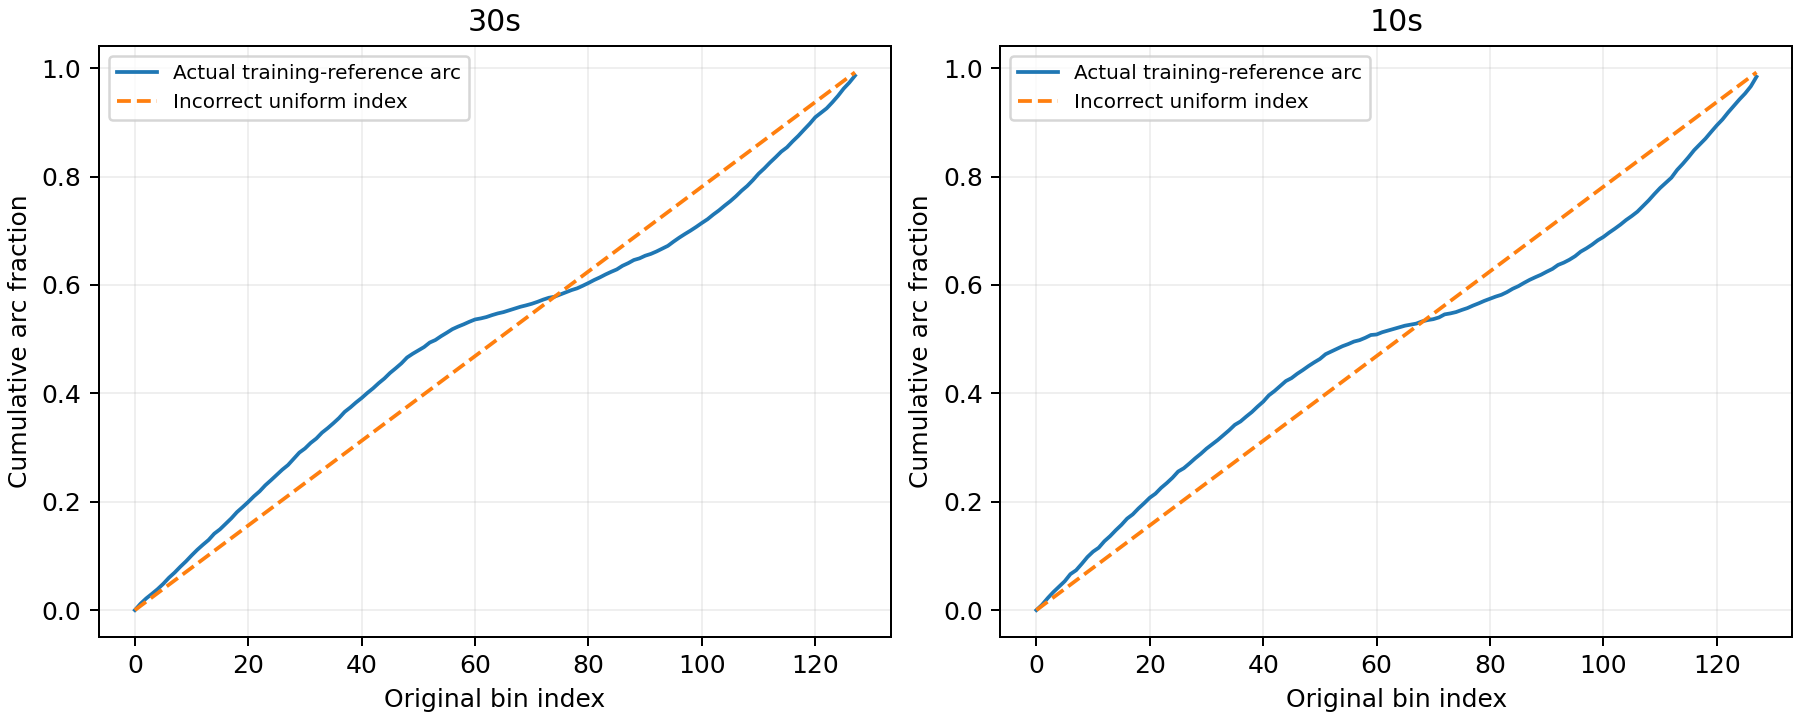
\includegraphics[width=\linewidth]{reference_coordinates.png}

The intensity objective remains
\[
J=\sum_{k,i}\left[\frac{I_{i,k}^{\rm pred}-I_{i,k}^{\rm obs}}{T_k^{\rm obs}}\right]^2.
\]
Three cone parameters, one brightness scale and one starting offset are fitted, plus correction parameters. No 16-parameter phase deformation. Optics, fixed gains/T, NA 0.38--1.3 and cycle selection remain unchanged (304/217 traversals). Training and test averages use alternate traversals.

\textbf{Numerical check.} A deliberately nonuniformly sampled synthetic model curve produces channel RMS 0.11364 when incorrectly matched by uniform indices. The corrected coordinate method reduces this to \(1.54\times10^{-5}\), with the remaining difference due to finite reference interpolation. Increasing reference interpolation subdivisions from 32 to 128 changes fractions by less than \(10^{-11}\). The selected finite non-Richard fits are refined at 8192 simulated segments; comparison at 16384 changes intensities by less than \(4\times10^{-8}T_{\max}\).

\textbf{Search and comparisons.} Each ordinary model/window used 18--19 coarse starts; the complex model used 24, across both directions, including nested zero/additive seeds and varied geometry. Selected none/additive/complex fits converge and beat their nested training baselines. Local search is not a global optimality certificate. Earlier flexible-phase controls use the same unchanged observations and still have lower held-out channel errors for the three original model families. That does not establish better physical angles. The coordinate repair changes recovered geometry materially even where the score changes modestly.

\newpage
{\Large Brightness constraint and the remaining Richard degeneracy}

For the fixed circular-excitation model,
\[
S_i=a_0^2\sin^2\theta\,q_i(\theta,\phi),\qquad
\sum_iS_i=4a_0^2\sin^2\theta(A_F+B_F\sin^2\theta).
\]
A sphere-circle inversion can use this total-intensity law at the recovered/projected orientations, plus the channel pair-sum condition. It must not choose an independent brightness per point. Time order supports phi unwrapping but does not by itself determine theta reflection branches at an equator crossing; those choices require continuity and physical-consistency checks. This report repairs correspondence only; it does not add new inverse-fit constraints.

Richard's model has another potential degeneracy even in a forward cone fit. Write \(S_i=a_0^2 f_i\), then
\[
I_i=a_0^2f_i+(a_0C_i)\sqrt{f_i}=\alpha f_i+K_i\sqrt{f_i},
\qquad \alpha=a_0^2,\quad K_i=a_0C_i.
\]
For positive alpha this is exactly the same model, with no additional degrees of freedom. The optimizer can reduce alpha toward zero while keeping K finite, which sends C to infinity. The original 10 s coefficient fit exhausted its refinement budget along this direction. Reparameterizing and searching nine starts converges to \(\alpha\approx6.7\times10^{-15}\), confirming the limiting tendency. Its predicted curve is well defined as a limit, but its separated signal/interference amplitudes are not a stable correction. The earlier numerical lower bound on brightness merely truncates this direction.

For 30 s the selected reparameterized solution has finite \(\alpha\approx0.01063\). Its physical adequacy still requires independent constraints. The bounded additive-plus-interference model instead uses
\[
I_i=S_i+B_i+2\rho_i\sqrt{B_iS_i},\quad |\rho_i|\leq1,
\quad B_{\rm total}\leq0.95\min T_{\rm train}.
\]
A finite background budget bounds its effective coefficients. These channel-wise bounds are necessary physical restrictions but do not establish realization by one common optical field.

\textbf{Interpretation.} The correspondence bug is repaired. The bounded-interference model now gives the smallest errors among these four corrected fixed-correspondence fits, but substantial mismatch remains. The result supports testing intensity/physical-budget constraints in the inverse-circle approach next, without claiming that current fitted angles are established or that flexible matching is physically superior.

Scripts, input-coordinate arrays, fit trials, predictions, resolution checks and Richard limiting analysis are saved in model\_comparison/corrected\_arc/. No commit or push.
\end{document}
